\documentclass[UKenglish,10pt]{beamer}
\usepackage{amsmath, amsfonts, amssymb}
\usepackage{pgf, tikz, bbm, svn}
\usepackage[latin1]{inputenc}
\usepackage{listings}

\lstset{language=C++, basicstyle=\tiny}
\newcommand{\Code}[1]{\texttt{#1}}


\usefonttheme{professionalfonts}

\definecolor{sintefblue}{rgb}{0.0,0.2,0.4}
\definecolor{dr}{rgb}{0.6,0.0,0.0}
\definecolor{dg}{rgb}{0.0,0.3,0.0}
\definecolor{db}{rgb}{0.0,0.0,0.5}
\setbeamercolor{uppercol}{fg=white,bg=sintefblue!80}
\setbeamercolor{lowercol}{fg=orange,bg=black!15}

\newcommand{\COto}{CO\ensuremath{_\mathsf{2}}}
\newcommand{\Tensor}[1]{\ensuremath{\mathsf{#1}}}
\newcommand{\Vector}[1]{\ensuremath{\boldsymbol{#1}}}
\newcommand{\Matrix}[1]{\ensuremath{\boldsymbol{#1}}}
\newcommand{\T}        {\ensuremath{\mathsf{T}}}
\newcommand{\Grad}     {\ensuremath{\nabla}}

\newcommand{\dunemod}[1]{\textsl{dune-{#1}}}
\newcommand{\opmmod} [1]{\textsl{opm{#1}}}
\newcommand{\dumux}    {DuMu\ensuremath{^{\mathrm X}}}

\def\bfK{{\bf K}}
\def\bfv{{\bf v}}
\def\bfn{{\bf n}}


\DeclareMathOperator{\Div}{div}




\usepackage{listings}
\usepackage{color}
\usepackage{textcomp}
\definecolor{listinggray}{gray}{0.9}
\definecolor{lbcolor}{rgb}{0.95,0.95,0.95}
\definecolor{lightgray}{gray}{0.3}
\lstset{%
  xleftmargin= 4pt,
  xrightmargin=4pt}
\lstdefinelanguage{MRST}{%
  alsoletter={...},%
  morekeywords={%                             % keywords
  break,case,catch,continue,elseif,else,end,for,function,global,%
  if,otherwise,persistent,return,switch,try,while,...},%
  comment=[l]\%,%                             % comments
  morecomment=[l]...,%                        % comments
  morestring=[m]',%                           % strings
}[keywords,comments,strings]%
\lstset{
  backgroundcolor=\color{lbcolor},
  tabsize=4,
  rulecolor=,
  language=MRST,
  basicstyle=\small,
  upquote=true,
  aboveskip={0.5\baselineskip},
  columns=flexible,
  showstringspaces=false,
  extendedchars=true,
%  breaklines=true,
  prebreak = \raisebox{0ex}[0ex][0ex]{\ensuremath{\hookleftarrow}},
  frame=single,
  showtabs=false,
  showspaces=false,
  showstringspaces=false,
  identifierstyle=\ttfamily,
  keywordstyle=\color[rgb]{0,0,1},
  commentstyle=\color[rgb]{0.133,0.545,0.133},
  stringstyle=\color[rgb]{0.627,0.126,0.941},
}
\newcommand{\mcode}[1]{\lstinline|#1|}

\tikzset{Workflow Stage/.style=%
        {rectangle, draw=blue!50, fill=blue!20, thick, %
         text width=35mm}}


\title{Upscaling}
\author[Atgeirr F. Rasmussen]{Atgeirr Fl{\o} Rasmussen}
\institute[SINTEF]{SINTEF ICT, Dept. Applied Mathematics}
\date[2017--01--25]{25th January 2017}

%%%%%%%%%%%%%%%%%%%%%%%%%%%%%%%%%%%%%%%%%%%%%%%%%%%%%%%%%%%%%%%%%%%%%%%%%%%%%%

\begin{document}


%============================================
\section{Upscaling}
%============================================



%--------------------
\begin{frame}
  \frametitle{Upscaling, what and why?}

  Upscaling means computing \emph{effective parameters} for a coarse
  scale simulation from fine-scale properties.
  \bigskip

  Examples include porosity, permeability, relative permeability,
  capillary pressure.
  \bigskip

  \includegraphics[width=\textwidth]{figs/OPM-upscaling.png}

  Upscaling is popular because:
  \begin{enumerate}
  \item Porous media flows are multi-scale phenomena.
  \item Large number of grid cells are necessary for accuracy.
  \item Complex physics make problems hard to compute with high
    resolution in reasonable time.
  \end{enumerate}
\end{frame}



%--------------------
% \begin{frame}
%   \frametitle{Alternatives to upscaling}

%   Recent \emph{multi-scale} methods can be viewed as an alternative to upscaling.
%   \bigskip

%   Example: Multiscale mixed FEM methods.
%   \includegraphics[width=0.9\textwidth]{figs/nornePartitionWithCells}

%   Compared to permeability upscaling:
%   \begin{itemize}
%   \item coarse scale basis functions resolve fine-grid effects better
%   \item may recompute (some) basis functions when flow patterns change
%   \item much greater coarse block flexibility
%   \end{itemize}
% \end{frame}



%--------------------
\begin{frame}
  \frametitle{Single-phase upscaling}
  In single-phase upscaling we seek to compute \emph{effective
    coarse-scale permeabilities} by solving fine-scale flow problems.

  \begin{columns}[c]
    \column{0.6\textwidth}
    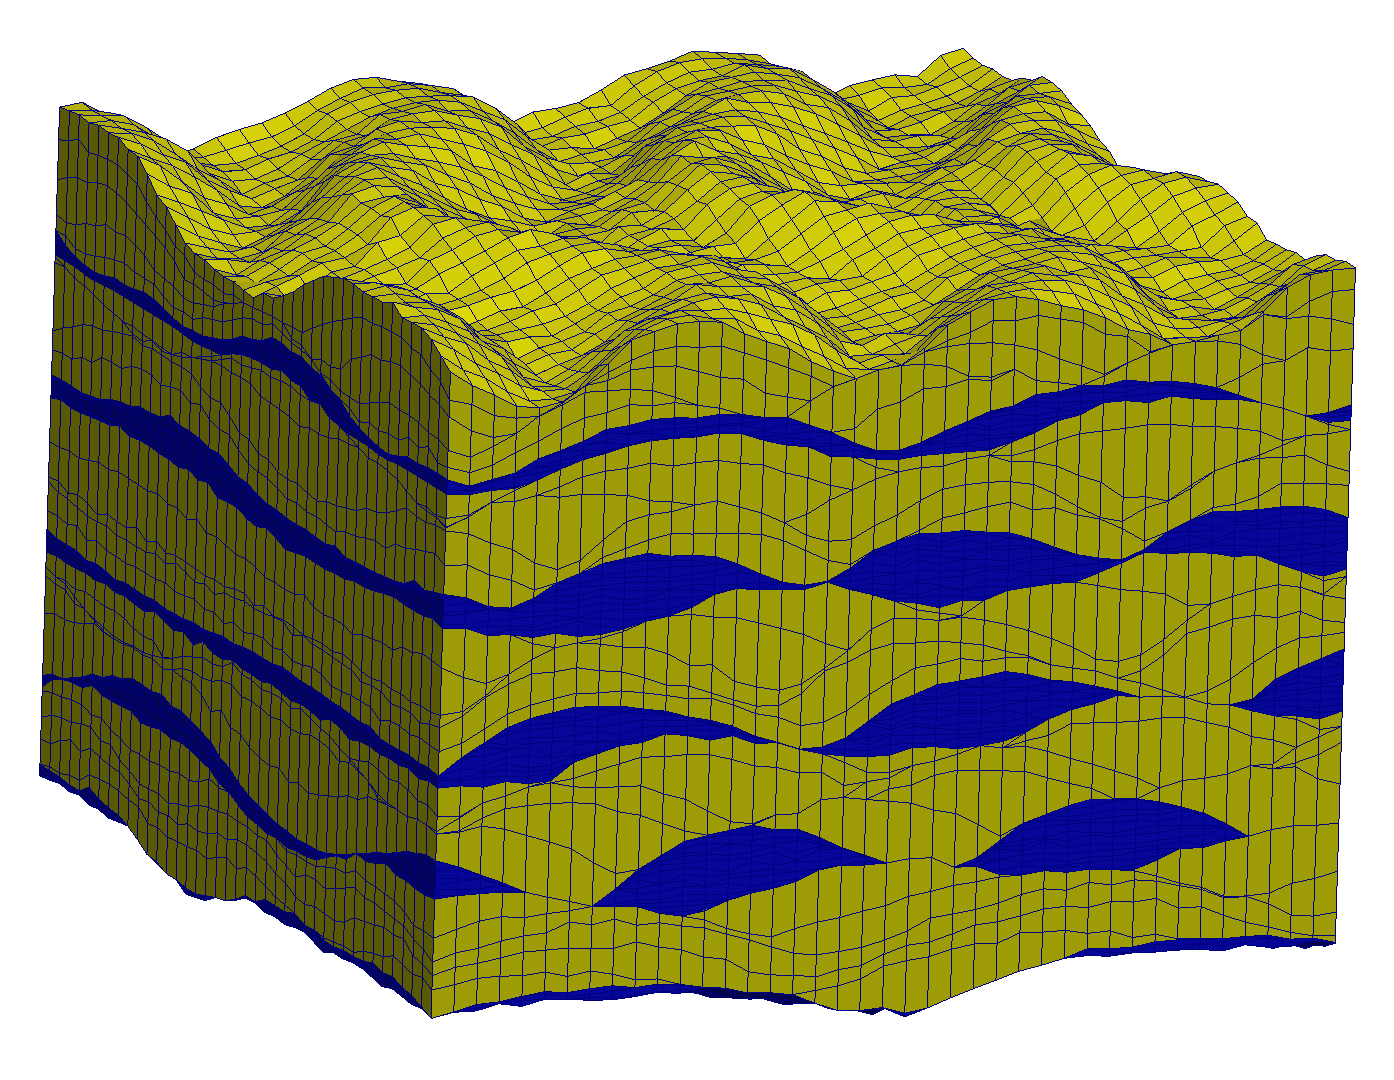
\includegraphics[width=\textwidth]{figs/wave_orig}
    \column{0.4\textwidth}
    Fine-scale permeability field.
  \end{columns}
  89791 cells, approximately $40 \times 40 \times 6$ cm, upscaled permeability
  \[
  \bfK_{eff} = 
  \begin{pmatrix}
    156.11 & 0 & 0 \\ 
    0 & 161.81 & 0 \\
    0 & 0 & 31.25 \\
  \end{pmatrix}
  \]
\end{frame}



%--------------------
\begin{frame}
  \frametitle{Flow-based upscaling approach}
  For a unit-sqare fine-scale domain $[0,1]^2$, solve the
  single-phase pressure equation with boundary conditions:

  \begin{columns}
    \column{0.3\textwidth}
    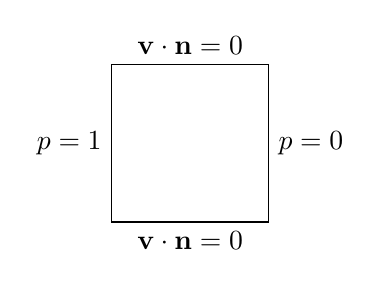
\begin{tikzpicture}
      \draw (0,0)
      -- node[below]{$\bfv\cdot\bfn = 0$} (2,0)
      -- node[right]{$p = 0$} (2,2)
      -- node[above]{$\bfv\cdot\bfn = 0$} (0,2)
      -- node[left]{$p = 1$} (0,0);
    \end{tikzpicture}
    \column{0.7\textwidth}
    \begin{align*}
      \nabla\cdot\bfv  & = 0 \\
      \bfv & = -\bfK\nabla p \\
    \end{align*}
  \end{columns}
  \bigskip

  From solution, compute average velocity over boundaries and estimate
  $\bfK_{eff}$ for the block (x direction) from Darcy's law. Repeat for
  other directions.
  \bigskip

  To apply this method, the domain must be reasonably close to a shoe-box.
\end{frame}



%--------------------
\begin{frame}
  \frametitle{Other boundary conditions}
  Alternative boundary conditions are possible:

  \begin{columns}
    \column{0.5\textwidth}
    \begin{tikzpicture}
      \draw (0,0)
      -- node[below]{$p = 1 - x$} (2,0)
      -- node[right]{$p = 0$} (2,2)
      -- node[above]{$p = 1 - x$} (0,2)
      -- node[left]{$p = 1$} (0,0);
    \end{tikzpicture}
    \column{0.5\textwidth}
    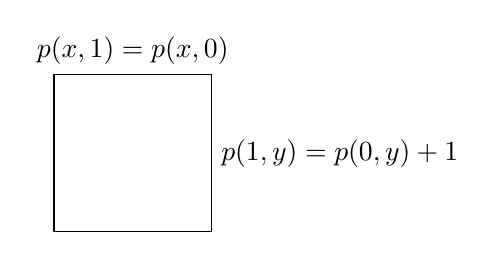
\begin{tikzpicture}
      \draw (0,0)
      -- (2,0)
      -- node[right]{$p(1,y) = p(0,y) + 1$} (2,2)
      -- node[above]{$p(x,1) = p(x,0)$} (0,2)
      -- (0,0);
    \end{tikzpicture}
  \end{columns}
  \bigskip

  For linear BCs (left) we get a full tensor, which may not be symmetric.
  \bigskip

  For periodic BCs (right) we get a full, symmetric tensor.
\end{frame}



%--------------------
% \begin{frame}[fragile]
%   \frametitle{The class \Code{SinglePhaseUpscaler}}

%   The class SinglePhaseUpscaler implements the method.

% \begin{lstlisting}
% ...

% /// Initializes the upscaler from parameters.
% void init(const parameter::ParameterGroup& param);

% /// Does a single-phase upscaling.
% /// @return an upscaled permeability tensor.
% permtensor_t upscaleSinglePhase();

% /// Compute upscaled porosity.
% /// @return total pore volume of all cells divided by total volume.
% double upscalePorosity() const;

% ...
% \end{lstlisting}
% \end{frame}



%--------------------
\begin{frame}
  \frametitle{Steady-state upscaling}

  We use steady-state upscaling to upscale relative permeabilities in
  the presence of nonzero capillary pressure.
  \bigskip

  Idea: Simulate till steady state reached, use the steady saturation
  distribution for upscaling computations.
  \bigskip

  To do this we simulate two-phase flow with:
  \begin{itemize}
  \item pressure BCs as for single-phase flow
  \item either periodic BCs for saturation, or some given inflow saturation
  \end{itemize}

  The resulting properties depend on the pressure drop! \\
  (transition from capillary limit to viscous limit)
\end{frame}



%--------------------
% \begin{frame}[fragile]
%   \frametitle{The class \Code{SteadyStateUpscaler}}

%   The template class \Code{SteadyStateUpscaler} implements the
%   algorithm.  The \Code{Traits} allow us (for example) to use either
%   scalar and tensor relative permeabilities.

% \begin{lstlisting}
% template <class Traits>
% class SteadyStateUpscaler : public UpscalerBase<Traits>
% {
%     std::pair<permtensor_t, permtensor_t>
%     upscaleSteadyState(const int flow_direction,
%                        const std::vector<double>& initial_saturation,
%                        const double boundary_saturation,
%                        const double pressure_drop,
%                        const permtensor_t& upscaled_perm);
%     const std::vector<double>& lastSaturationState() const;
%     double lastSaturationUpscaled() const;
%     ...
% };

% \end{lstlisting}

% \end{frame}




%--------------------
\begin{frame}
  \frametitle{Upscaling}
  \begin{itemize}
  \item Permeability (single-phase)
  \item Relative permeability (two-phase)
  \end{itemize}
  \bigskip

  This line of work started before OPM (first delivery 2006)

  \begin{columns}[c]
    \column{0.5\textwidth}
    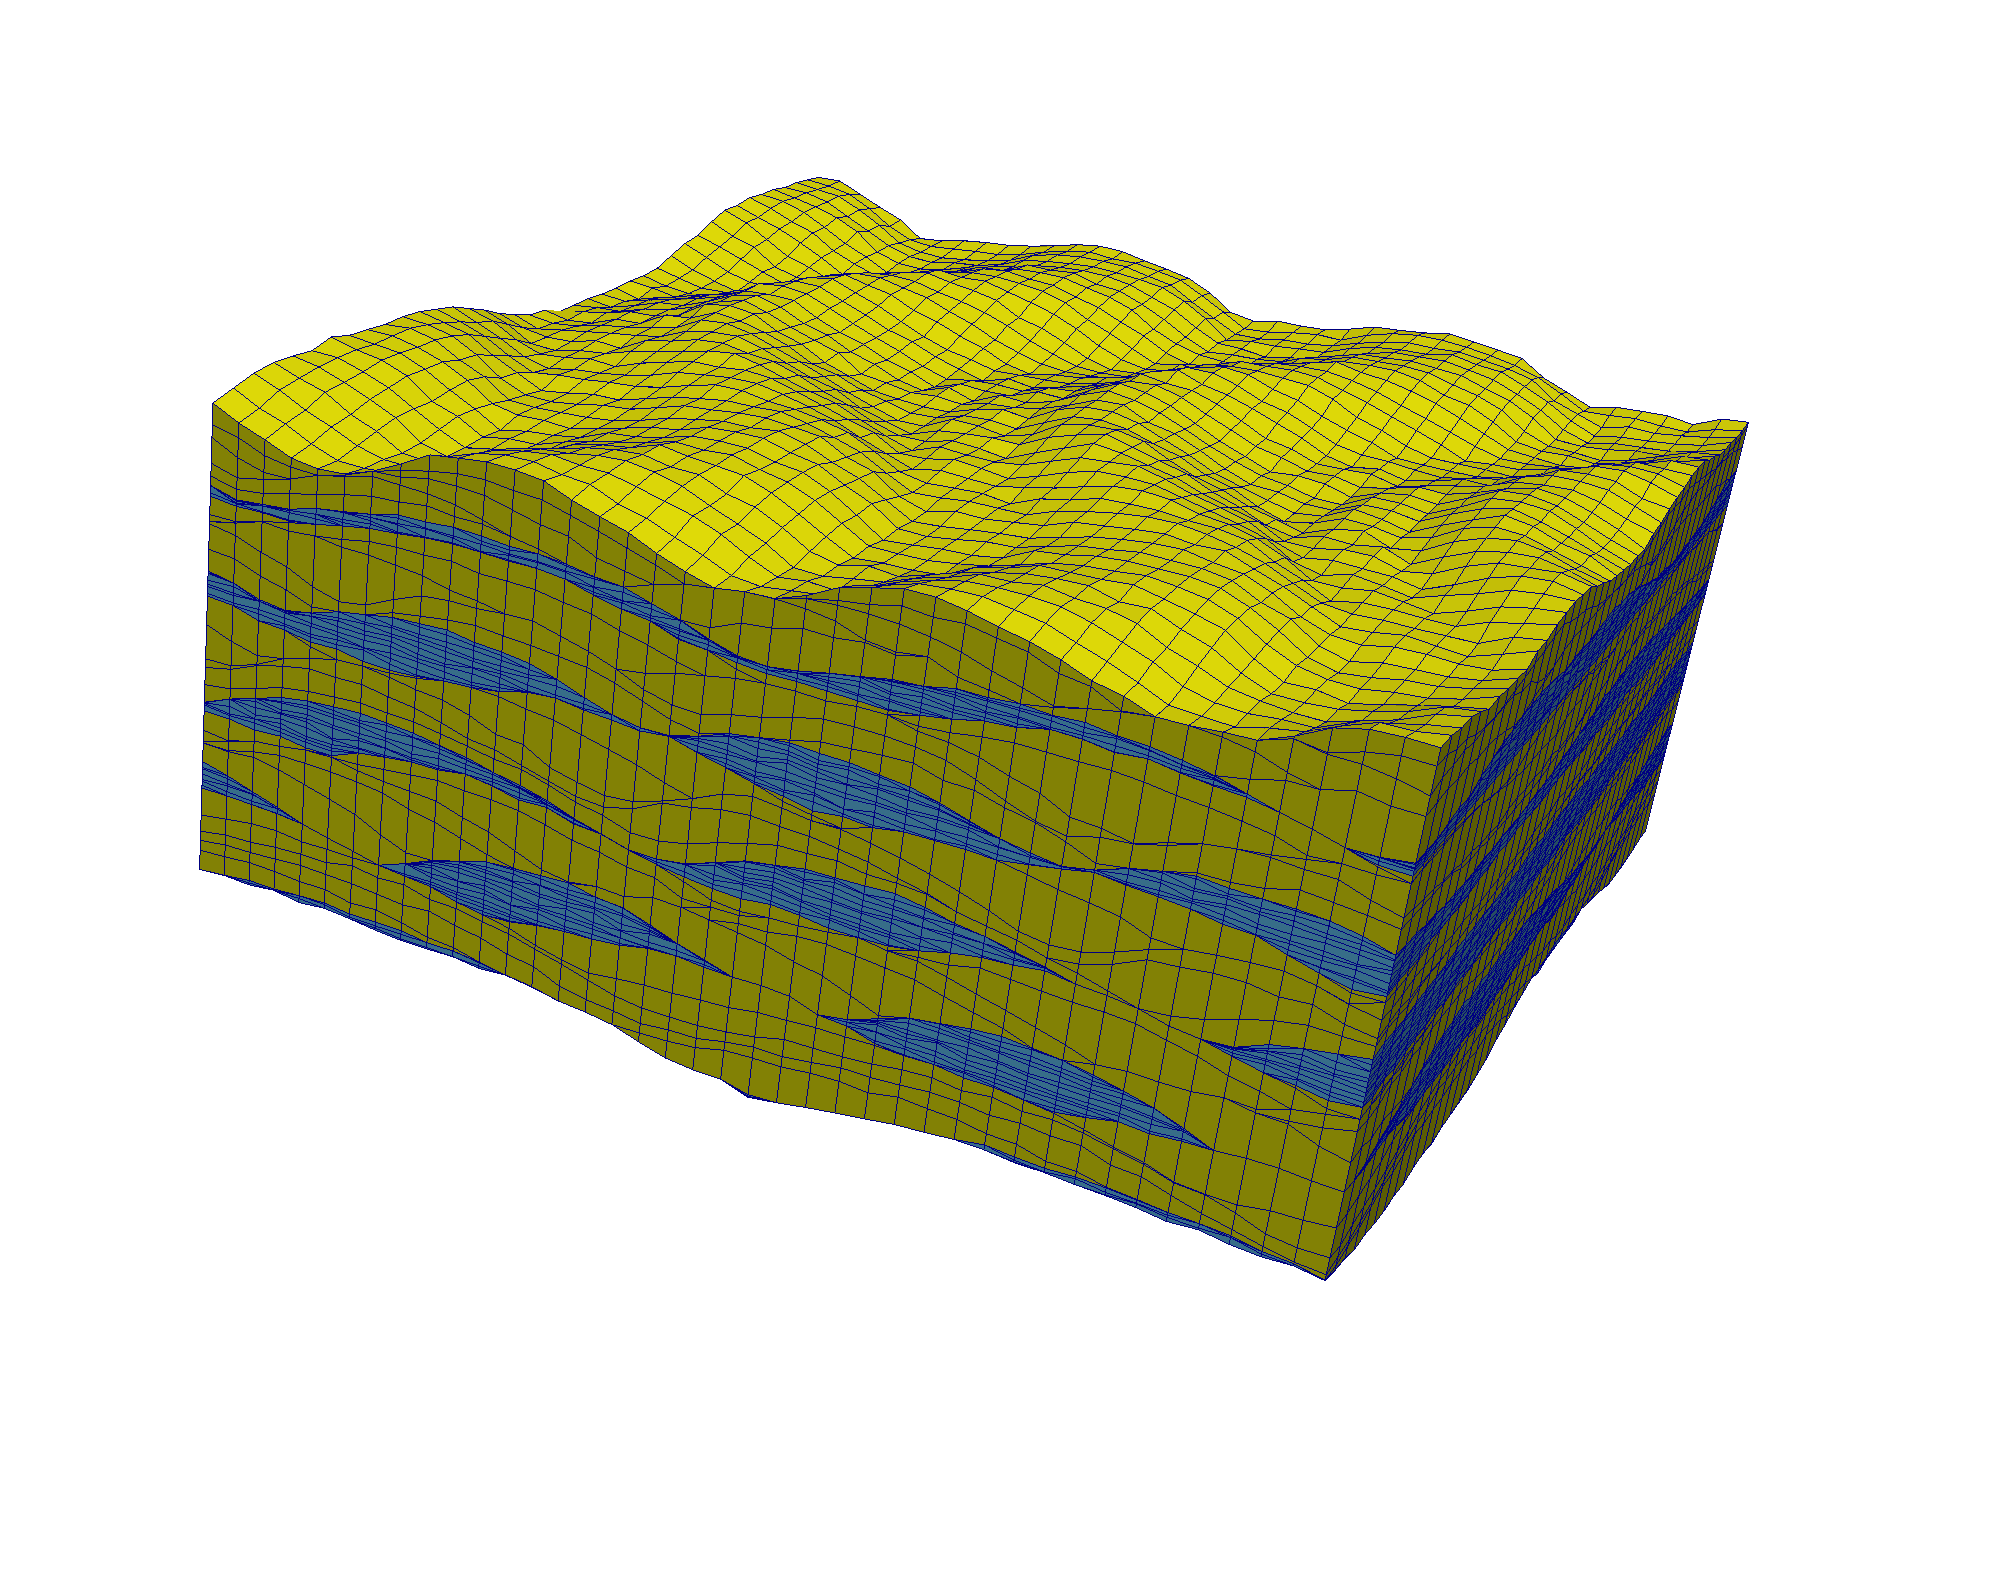
\includegraphics[width=1.2\textwidth]{figs/wave_orig_angled}
    \column{0.5\textwidth}
    \small
    \begin{equation*}
    \overline{K} =
    \left(
      \begin{array}{ccc}
        156.1 & 0 & 0 \\
        0 & 161.8 & 0 \\
        0 & 0 & 31.25
      \end{array}
    \right)
    \end{equation*}
    (using Fixed boundary conditions)
    \begin{equation*}
    \overline{K} =
    \left(
      \begin{array}{ccc}
        155.3 & -0.0872 & 0.1651 \\
        -0.0872 & 158.4 & 0.0052 \\
        0.1652 & 0.0052 & 29.09 
      \end{array}
    \right)
    \end{equation*}
    (using Periodic boundary conditions)
  \end{columns}
\end{frame}



%--------------------
\begin{frame}
  \frametitle{Upscaling: permeability}
  \begin{itemize}
  \item Flow-based: solve directional pressure problems
  \item Much more accurate than harmonic averaging etc.
  \item Mimetic discretization of pressure
  \item Linear solver: dune-istl AMG (or FastAMG)
  \item Fixed, Linear or Periodic boundaries
  \item Produces symmetric tensor (with periodic bondaries)
  \end{itemize}
  \bigskip

  In wide use in Statoil.
\end{frame}



%--------------------
\begin{frame}
  \frametitle{Upscaling: relative permeability}
  \begin{block}{Approach used: steady-state upscaling}
    \begin{itemize}
    \item Compute a steady-state for given configuration
    \item Depends on flow direction, pressure drop, initial saturation
    \item Compute upscaled perm based on phase mobilities
    \item Produces full tensor relperm as output
    \end{itemize}
  \end{block}

  \begin{block}{Computing steady states}
    Simple for CL, VL. Between those, must simulate.
    \begin{itemize}
    \item Two-phase incompressible, immiscible flow
    \item Include capillary pressure, gravity
    \item Fixed, Linear or Periodic bondaries
    \item Pressure: mimetic discretization, AMG
    \item Saturation: TPFA discretization, explicit or implicit Euler
  \end{itemize}
  \end{block}
\end{frame}

\end{document}